\documentclass[11pt, oneside]{article}   	% use "amsart" instead of "article" for AMSLaTeX format
\usepackage{amssymb}
\usepackage{commath} % Will load amsmath, used for \dif
\usepackage{physics}
\usepackage{tikz,tikz-3dplot}

\newcommand{\vect}[1]{\boldsymbol{#1}} % Uncomment for BOLD vectors.
%\newcommand{\vect}[1]{\vec{#1}} % Uncomment for ARROW vectors.

% --------------------------------------- Title Matter -----------------------------------------

\title{Derivation of the Differential Continuity Equation}
\author{Eric Mott}
\date{2015-10-11}

% --------------------------------------- Begin Document -----------------------------------------

\begin{document}
\maketitle 	% Places title matter

% --------------------------------------- Derivation -----------------------------------------

\section{Continuity Equation}

\begin{figure}
\centering
\tdplotsetmaincoords{305}{75}
    
    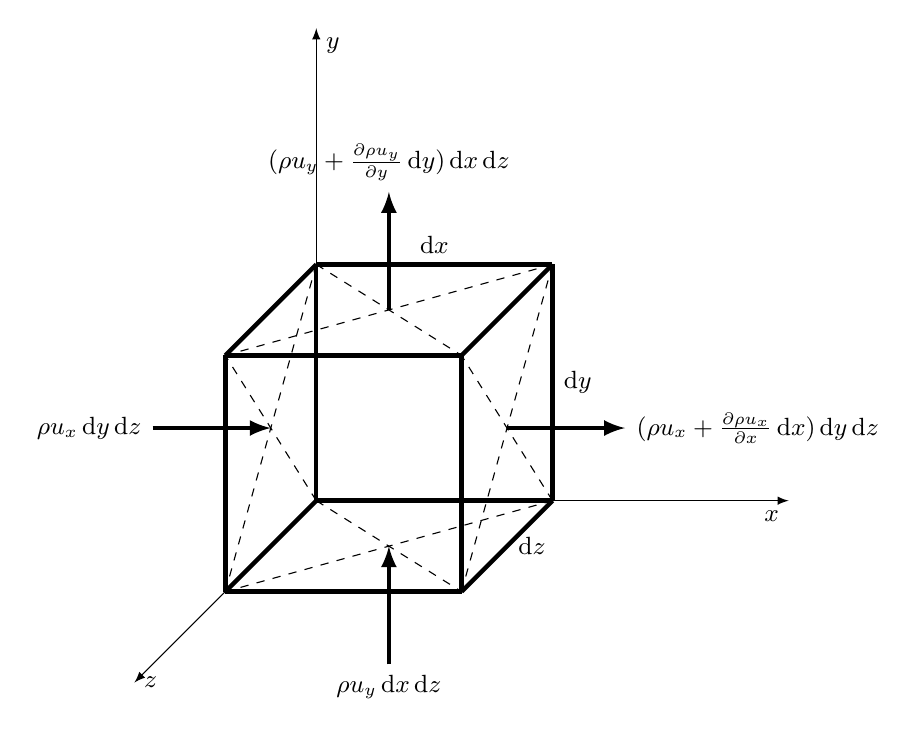
\begin{tikzpicture}[scale = 3]
        \tikzstyle{every node}=[font = \small]
        
        % x, y, and z axes
        \draw[-latex] (0,0,0) -- (2,0,0) node[anchor = north east] {$x$};
        \draw[-latex] (0,0,0) -- (0,2,0) node[anchor = north west] {$y$};
        \draw[-latex] (0,0,0) -- (0,0,2) node[anchor = west] {$z$};
        
        % Edges of elemental control volume
        \draw [ultra thick] (0,0,0) -- (1,0,0);
        \draw [ultra thick] (0,0,0) -- (0,1,0);
        \draw [ultra thick] (0,0,0) -- (0,0,1);
        \draw [ultra thick] (0,1,0) -- (1,1,0) node[midway, anchor = south] {$\dif x$};
        \draw [ultra thick] (1,1,0) -- (1,0,0) node[midway, anchor = west] {$\dif y$}; 
        \draw [ultra thick] (1,0,0) -- (1,0,1) node[midway, anchor = west] {$\dif z$};
        \draw [ultra thick] (0,1,1) -- (0,1,0);
        \draw [ultra thick] (1,1,1) -- (1,1,0);
        \draw [ultra thick] (1,1,1) -- (1,0,1);
        \draw [ultra thick] (1,1,1) -- (0,1,1);
        \draw [ultra thick] (1,0,1) -- (0,0,1);
        \draw [ultra thick] (0,1,1) -- (0,0,1);
        
        \draw [dashed] (0,0,0) -- (0,1,1);
        \draw [dashed] (0,1,0) -- (0,0,1);
        \draw [dashed] (1,0,0) -- (1,1,1);
        \draw [dashed] (1,1,0) -- (1,0,1);
        \draw [dashed] (0,0,0) -- (1,0,1);
        \draw [dashed] (1,0,0) -- (0,0,1);
        \draw [dashed] (0,1,0) -- (1,1,1);
        \draw [dashed] (1,1,0) -- (0,1,1);
        
        % Mass flow vectors
        \draw [ultra thick, -latex] (-0.5, 0.5, 0.5) -- (0.0, 0.5, 0.5) node[at start, anchor = east] {$ \rho u_x \dif y \dif z $}; % mass flow in, x-direction
        \draw [ultra thick, -latex] ( 1.0, 0.5, 0.5) -- (1.5, 0.5, 0.5) node[anchor = west] {$ ( \rho u_x + \pdv{\rho u_x}{x} \dif x ) \dif y \dif z $}; % mass flow out, x-direction
        \draw [ultra thick, -latex] ( 0.5,-0.5, 0.5) -- (0.5, 0.0, 0.5) node[at start, anchor = north] {$ \rho u_y \dif x \dif z $}; % mass flow in, y-direction    
        \draw [ultra thick, -latex] ( 0.5, 1, 0.5) -- (0.5, 1.5, 0.5) node[anchor =  south] {$ ( \rho u_y + \pdv{\rho u_y}{y} \dif y ) \dif x \dif z $}; % mass flow out, x-direction
        
    \end{tikzpicture}
    
\end{figure}

Starting with the first principle of conservation of mass:

\begin{equation}
\text{time rate change in mass} = \text{mass transfer in} - \text{mass transfer out}
\end{equation}

\noindent 
This can be expressed mathematically as:

\begin{equation}
\pdv{m}{t} = \dot{m}_{in} - \dot{m}_{out}
\end{equation}

\begin{equation}
\pdv{m}{t} = (\rho A u)_{in} - (\rho A u)_{out}
\end{equation}

\noindent
For the infinitesimal control volume defined by lengths $\dif x$, $\dif y$, and $\dif z$, mass can be expressed in terms of the density, $\rho$, as:

\begin{equation}
m = \rho \dif x \dif y \dif z
\end{equation}

\begin{equation}
\pdv{\rho}{t} \dif x \dif y \dif z = \dot{m}_{in} - \dot{m}_{out}
\end{equation}

\begin{equation}
\frac{\Dif \rho}{\Dif t}   = - \rho \div \vect{u}
\end{equation}

\end{document}